\chapter{Introduction}
\label{cha:introchap}

In 1905, Einstein published a paper on the photoelectric effect \cite{einstein1905}, for which he later received the Noble Prize. The effect shows when light is shined on an object an electron can be ionized from an atom, molecule, or solid by absorbing a photon with a sufficiently high energy. With the advent of the laser in 1960, it became possible to focus coherent light tight enough to allow the ionization process to occur not only by absorbing one but many photons in rapid succession leading to a process known as multiphoton ionization \cite{goppertmayer1931}. Since then, laser intensities have increased to the point where the superposition of the electric field of the laser with the attractive potential produced by a nucleus can create a barrier and allow the electron to tunnel and ionize from the atom \cite{keldysh1965}. Furthermore, depending on various laser parameters, the electron that tunneled through the barrier can interact with the laser field and recombine with the residual ion. During the recombination process, photons are released at harmonics of the driving laser's central frequency. This process can convert a large numbers of infrared (IR) photons into a single X-ray photon in a process known as high-order harmonic generation (HHG) \cite{franken1961,lewenstein1994,corkum1994}. HHG is one method that allows for the production of bright X-ray laser pulses with pulse durations as short as tens of attoseconds \cite{zhao2012,chen2014} ($10^{-18}$ sec). Recent developments have allowed for the generation high-order harmonics using not only linearly polarized lasers but also lasers or combination of lasers with other polarizations \cite{fleischer2014,pisanty2014,kfir2015,fan2015,hickstein2015}. Such pulses provide the tools necessary for the imaging of electron dynamics on their fundamental time scale \cite{krausz2009}. 

Einstein's photoelectric effect mostly considered continuous wave (CW) light that produced a near delta function like energy distribution. These CW lasers are good for precision energy measurements, however, their time resolution it greatly limited. The recent advances in attosecond pulse technology have strongly decreased the interaction time allowing for the imaging of (attosecond) electron dynamics at the cost of energy bandwidths of the pulses on the order of several eVs. The largely increased pulse bandwidth, however, leads to many competing pathways of ionization that can involve different numbers of photons complicating the ionization process. The photoelectron angular distributions (PAD) produced by such pulses contain complex shapes that encode features of the target's initial wavefunction, ionization cross sections for each process, the ionizing pulse, and the various competing pathways to ionization. This naturally raises the question of how can one backtrack all of this information from such a PAD signal?

In this thesis, we will explore methods to understand and image the motion of electrons on ultrashort time scales from ionization signals and photoelectron angular distributions. Then, we will also analyze how intense IR light can cause that electrons are being trapped in highly excited states although the absorption of a single additional photon would lead to ionization. Finally, the focus will be turned to a new numerical method that we are developing to study two fully correlated electrons interacting with each other and an ultrafast laser pulse. 

%%%%%%%%%%%%%%%%%%%%%%%%%%%%%%%%%%%%%%%%%%%%%%%%%%%%%%%%%%%%%%%%%%%%%%%%%%%%%%%%%%%%%%%%%%%%%%%%%%%%%%%%%%%%%%%%%%
%%%%%%%%%%%%%%%%%%%%%%%%%%%%%%%%%%%%%%%%%%%%%%%%%%%%%%%%%%%%%%%%%%%%%%%%%%%%%%%%%%%%%%%%%%%%%%%%%%%%%%%%%%%%%%%%%%
%%%%%%%%%%%%%%%%%%%%%%%%%%%%%%%%%%%%%%%%%%%%%%%%%%%%%%%%%%%%%%%%%%%%%%%%%%%%%%%%%%%%%%%%%%%%%%%%%%%%%%%%%%%%%%%%%%
%%%%%%%%%%%%%%%%%%%%%%%%%%%%%%%%%%%%%%%%%%%%%%%%%%%%%%%%%%%%%%%%%%%%%%%%%%%%%%%%%%%%%%%%%%%%%%%%%%%%%%%%%%%%%%%%%%
%%%%%%%%%%%%%%%%%%%%%%%%%%%%%%%%%%%%%%%%%%%%%%%%%%%%%%%%%%%%%%%%%%%%%%%%%%%%%%%%%%%%%%%%%%%%%%%%%%%%%%%%%%%%%%%%%%
\section{Attosecond time scale}
The idea of an attosecond (1 as = $10^{-18}$ sec) is difficult to wrap ones mind around. Some perspective can be gained by noting that there are more attoseconds in a single second than seconds in the lifetime of the universe. At this ultrashort time scale, nearly all motion in an atom, molecule or solid is frozen. Only the motion of electrons, particularly that in atoms as visualized in Fig.~\ref{fig:time_scales}, is non-negligible. With laser technology recently reaching pulse durations with sub 100 attosecond pulse widths \cite{zhao2012,chen2014}, it is becoming possible to ``image'' electrons as they move around inside of atoms and molecules. One approach to imaging electron motion will be presented in this thesis (see  Chap.~\ref{cha:imaging_wave_packets_with_photoelectrons}).

\begin{figure}[!ht]
\centering
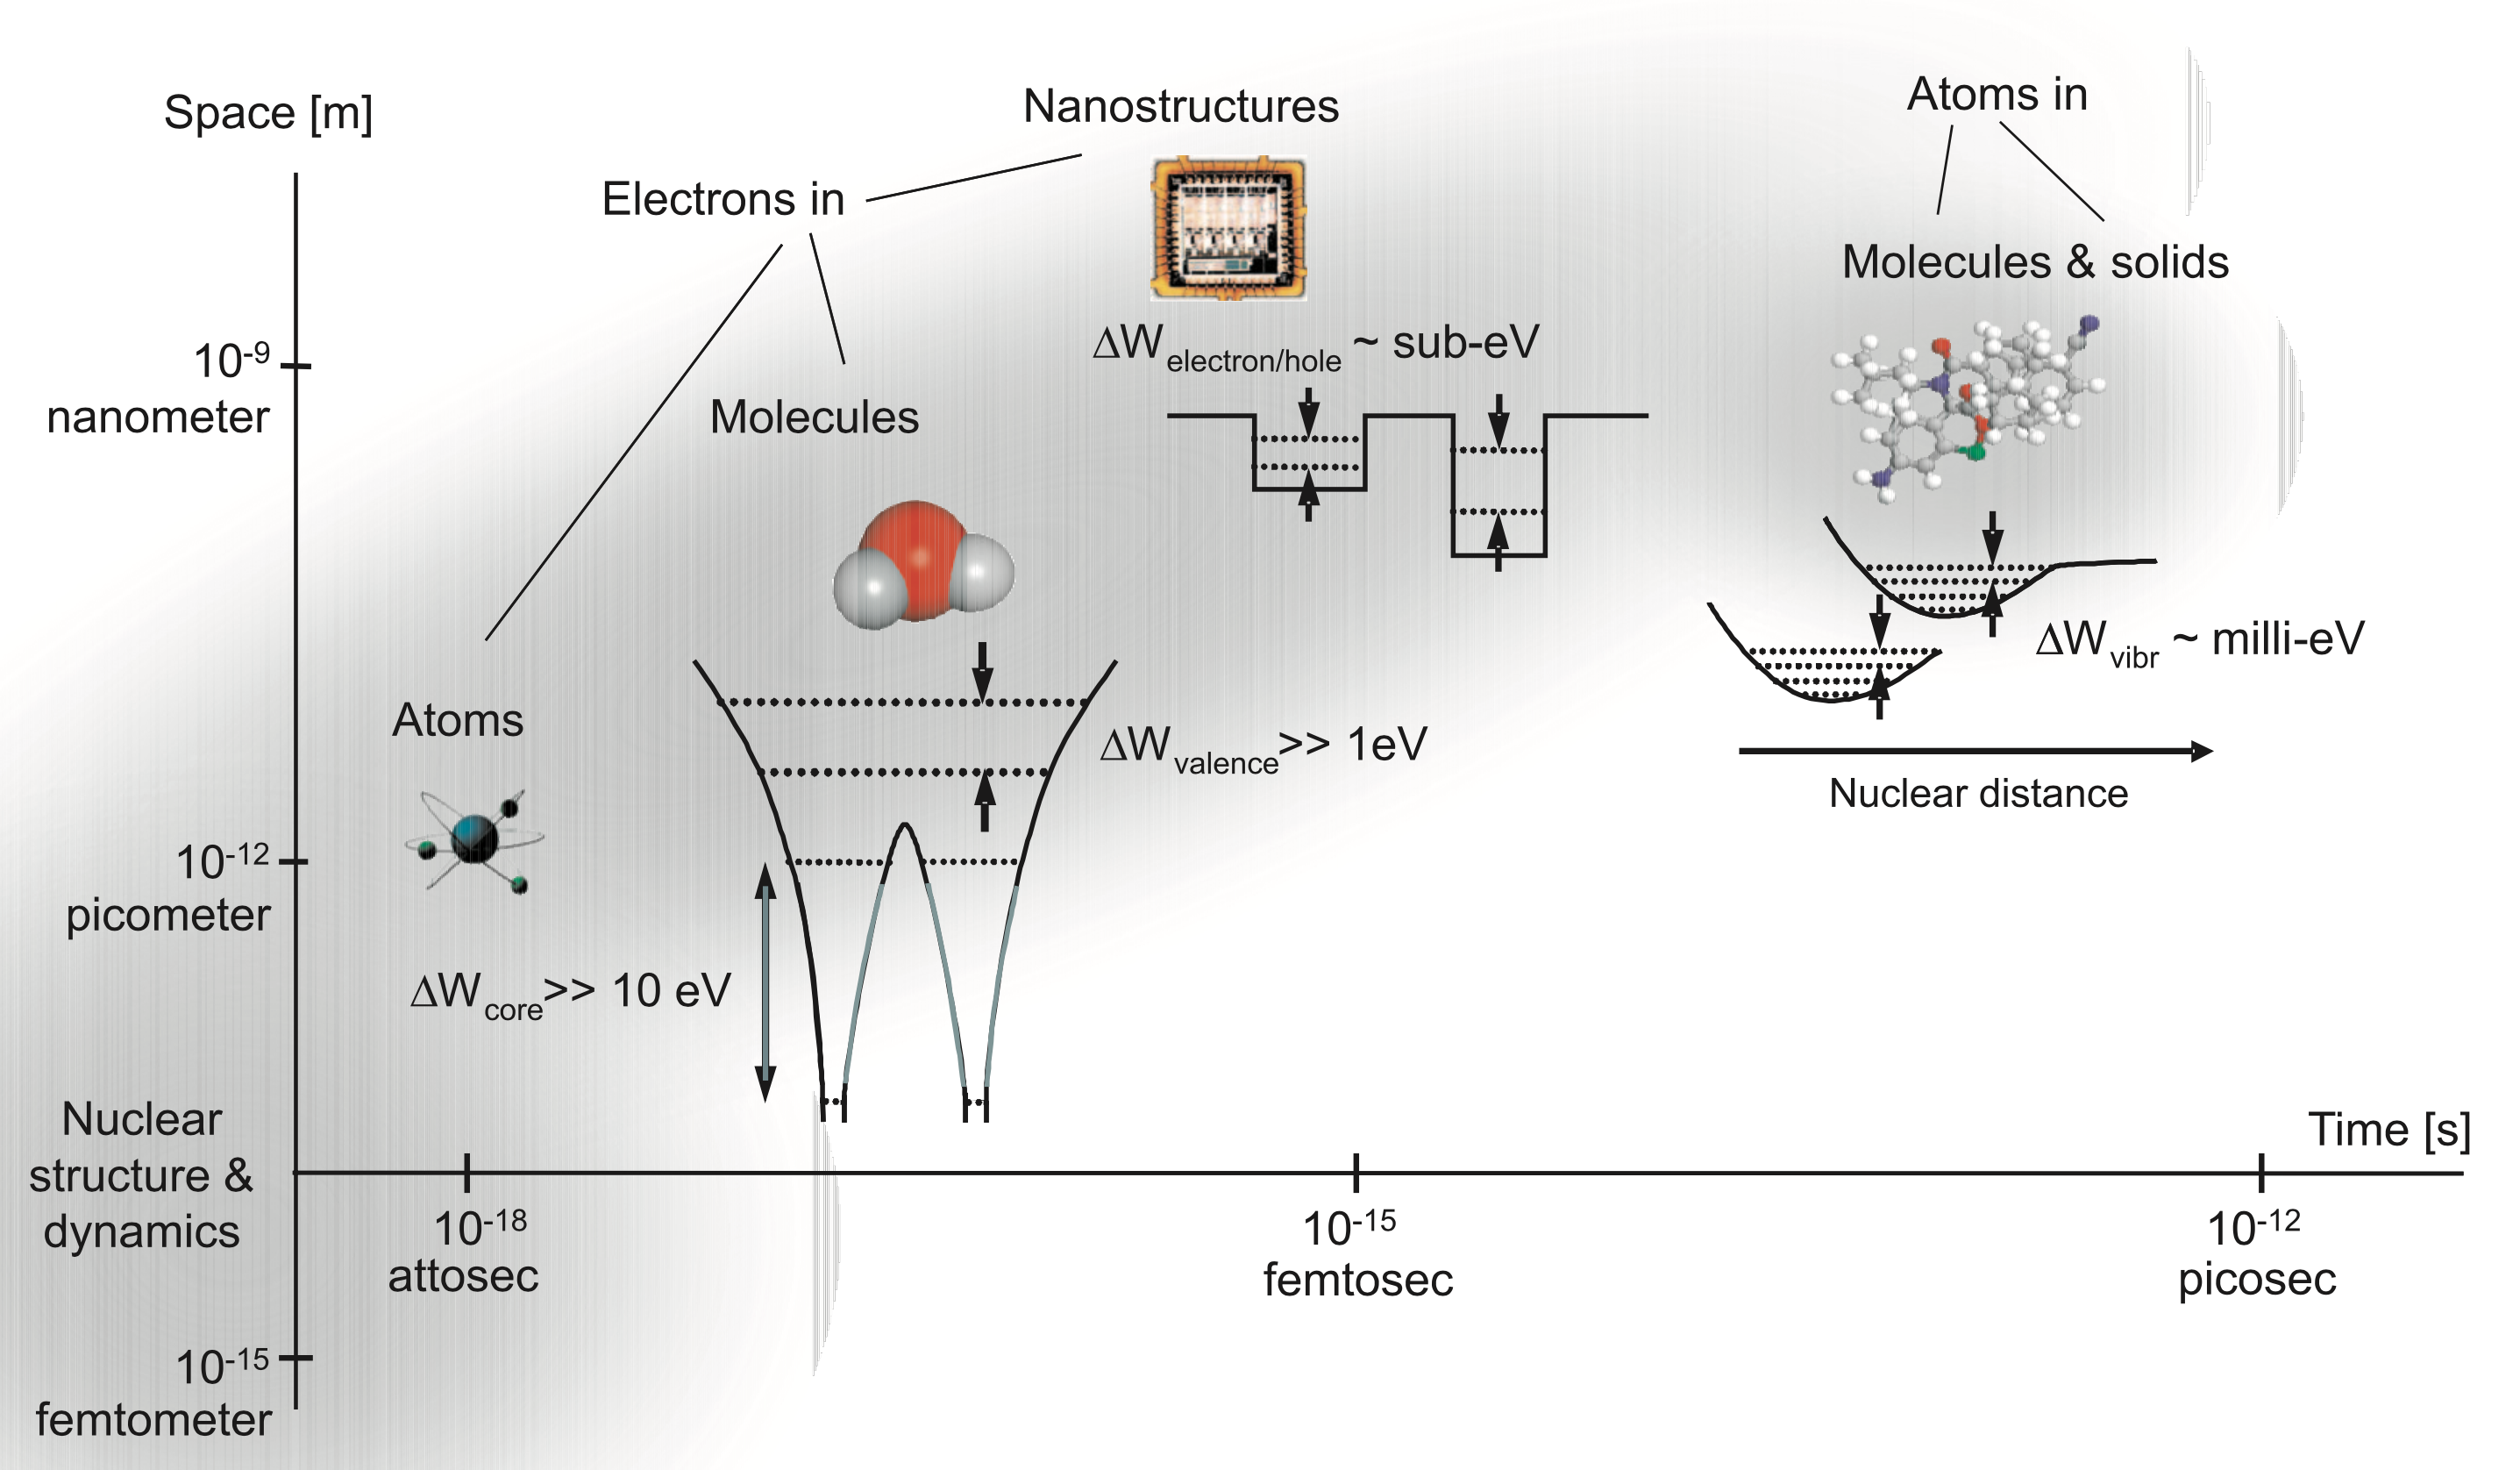
\includegraphics[width=0.8\columnwidth]{figs/Intro/time_scales.png}
\caption{\label{fig:time_scales} Relevant space and time scales present in ultrafast physics. (Figure from \cite{krausz2009})
}
\end{figure}

%%%%%%%%%%%%%%%%%%%%%%%%%%%%%%%%%%%%%%%%%%%%%%%%%%%%%%%%%%%%%%%%%%%%%%%%%%%%%%%%%%%%%%%%%%%%%%%%%%%%%%%%%%%%%%%%%%
%%%%%%%%%%%%%%%%%%%%%%%%%%%%%%%%%%%%%%%%%%%%%%%%%%%%%%%%%%%%%%%%%%%%%%%%%%%%%%%%%%%%%%%%%%%%%%%%%%%%%%%%%%%%%%%%%%
%%%%%%%%%%%%%%%%%%%%%%%%%%%%%%%%%%%%%%%%%%%%%%%%%%%%%%%%%%%%%%%%%%%%%%%%%%%%%%%%%%%%%%%%%%%%%%%%%%%%%%%%%%%%%%%%%%
%%%%%%%%%%%%%%%%%%%%%%%%%%%%%%%%%%%%%%%%%%%%%%%%%%%%%%%%%%%%%%%%%%%%%%%%%%%%%%%%%%%%%%%%%%%%%%%%%%%%%%%%%%%%%%%%%%
%%%%%%%%%%%%%%%%%%%%%%%%%%%%%%%%%%%%%%%%%%%%%%%%%%%%%%%%%%%%%%%%%%%%%%%%%%%%%%%%%%%%%%%%%%%%%%%%%%%%%%%%%%%%%%%%%%
\section{Light sources}

The fields of ultrastrong and ultrafast physics rely on bright laser light to study and understand the behavior of matter on short time scales. The light used ranges from intense IR radiation, that can bend atomic and molecular potentials enough to allow electrons to tunnel into the continuum, to hard X-rays that can ionize multiple electrons with a single photon. The intense IR light is often produced  using Ti:sapphire or similar laser setups. In the following subsections, we will briefly describe the two major sources of ultrafast extreme ultraviolet (XUV) to X-ray sources and the applications they are designed for.

\subsection{High harmonic generation} % (fold)
\label{sub:high_harmonic_generation}
High harmonic generation (HHG) is a process that converts low-energy photons of intense IR laser pulses into high-energy photons of an X-ray laser pulse through a highly non-linear and non-perturbative process. The process is often understood through the so-called three step model shown in Fig.~\ref{fig:hhg_3_step} \cite{lewenstein1994,corkum1994,popmintchev2010}. First, the strong electric field of the IR laser bends the atomic Coulomb potential allowing for the electron to tunnel ionize. Next, the electron interacts with the field gaining energy and reversing direction when the oscillating field changes direction. Finally, the electron recombines with the ion releasing its energy in the form of a high-energy photon. For linearly polarized laser pulses, the emitted electrons have energies corresponding to $(2n+1)\omega$ where $n$ is an integer and $\omega$ in the central frequency of the driving laser pulse. 

\begin{figure}[!ht]
\centering
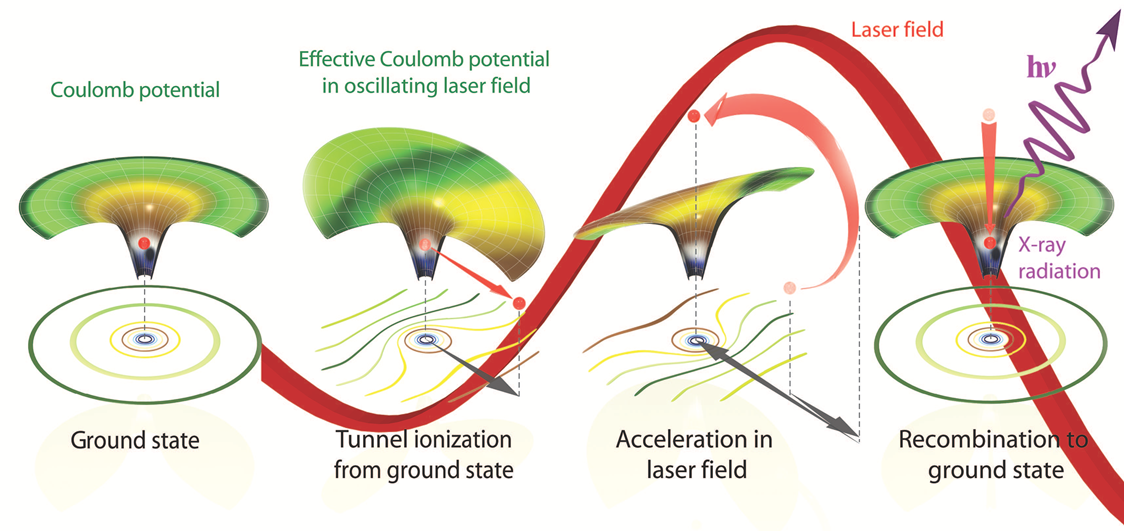
\includegraphics[width=0.8\columnwidth]{figs/Intro/HHG.png}
\caption{\label{fig:hhg_3_step} Schematics of the three step model in which an electron tunnel ionizes, is accelerated in the continuum by the driving laser and recombines with the remaining ion producing a high energy photon. (Figure from \cite{popmintchev2010})
}
\end{figure}


Nowadays, HHG sources can produce laser pulses with arbitrary polarization \cite{fleischer2014,pisanty2014,kfir2015,fan2015,hickstein2015}. The theoretical method for generating circularly polarized HHG sources was proposed more than two decades ago \cite{eichmann1995,long1995}. By using two counter rotating cicularly polarized IR lasers with frequencies $\omega$ and $2\omega$, a so called counter-rotating bi-circular laser pulse is produced. The three fold symmetry of the final laser pulse allows for the electron to recombine with the parent ion, something that is not possible with a circularly polarized pulse alone. The resulting HHG spectrum contains circularly polarized harmonics at energies of $(3n+1)\omega$ and  $(3n+2)\omega$ with alternating helices and no harmonic at energies of $3n\omega$. Since then, non-collinear methods of circularly polarized HHG \cite{hickstein2015} and methods for elliptically polarized harmonics \cite{barreau2018} have been demonstrated.

HHG sources have the advantage that they are compact table top setups. Additionally, the light produced is coherent and carrier-to-envelope phase locking can be achieved in certain cases, which make it possible to control the light produced in these sources. As a result, trains of attosecond long pulses can be generated \cite{kim2013}, and isolated pulses with a duration of only a few tens of attoseconds have been demonstrated \cite{zhao2012,chen2014}. For more details on HHG light sources, we refer to Ref.~\cite{popmintchev2010,chini2014}
% subsubsection high_harmonic_generation (end)

\subsection{Free electron lasers} % (fold)
\label{sub:free_electron_lasers}
Free electron lasers (FEL) differ significantly from HHG sources. Often located at large shared user facilities \cite{seddon2017}, they start with a high energy electron beam from an accelerator. The electron beam is then passed through an undulator consisting of alternating magnetic fields. The electrons oscillate back and forth leading to a phenomenon known as micro bunching and the generation of light. After leaving the undulator, the electron beam is dumped while an X-ray laser pulse propagates towards the experimental stations, as shown in Fig.~\ref{fig:FEL_diagram}. By tuning the spacing between the magnets, the frequency of the light can be changed. 

\begin{figure}[!ht]
\centering
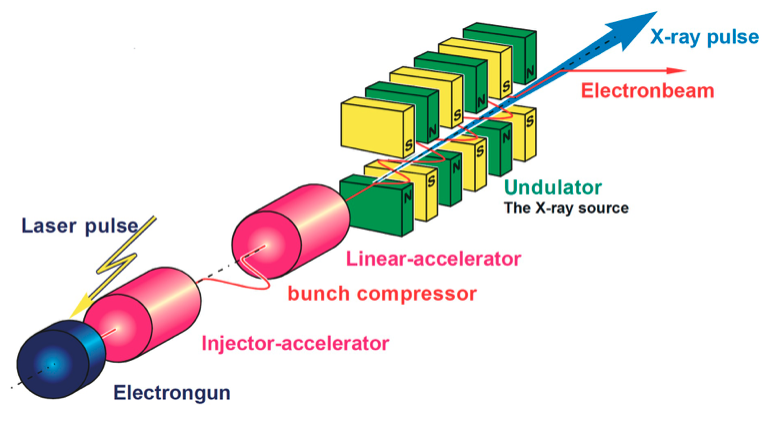
\includegraphics[width=0.8\columnwidth]{figs/Intro/FEL.png}
\caption{\label{fig:FEL_diagram} Schematics of an FEL laser showing the electron bunch production, undulator, and beam dump that are essential parts to generate an X-ray pulse. (Figure from \cite{rauschenbergerFEL})
}
\end{figure}

Due to the large amount of energy in an electron bunch, FEL sources are much brighter than HHG sources in the same frequency range. FEL can produce arbitrary polarized laser pulses \cite{ilchen2017} and pulses with a duration less than a femtosecond have been demonstrated \cite{marinelli2017}. The laser pulses, however, are only partially coherent and their shape varies widely from shot to shot limiting their application for effects that depend significantly on the control of the pulse parameters. For more details on FEL technology, see  \cite{seddon2017}.
% subsubsection free_electron_lasers (end)

%%%%%%%%%%%%%%%%%%%%%%%%%%%%%%%%%%%%%%%%%%%%%%%%%%%%%%%%%%%%%%%%%%%%%%%%%%%%%%%%%%%%%%%%%%%%%%%%%%%%%%%%%%%%%%%%%%
%%%%%%%%%%%%%%%%%%%%%%%%%%%%%%%%%%%%%%%%%%%%%%%%%%%%%%%%%%%%%%%%%%%%%%%%%%%%%%%%%%%%%%%%%%%%%%%%%%%%%%%%%%%%%%%%%%
%%%%%%%%%%%%%%%%%%%%%%%%%%%%%%%%%%%%%%%%%%%%%%%%%%%%%%%%%%%%%%%%%%%%%%%%%%%%%%%%%%%%%%%%%%%%%%%%%%%%%%%%%%%%%%%%%%
%%%%%%%%%%%%%%%%%%%%%%%%%%%%%%%%%%%%%%%%%%%%%%%%%%%%%%%%%%%%%%%%%%%%%%%%%%%%%%%%%%%%%%%%%%%%%%%%%%%%%%%%%%%%%%%%%%
%%%%%%%%%%%%%%%%%%%%%%%%%%%%%%%%%%%%%%%%%%%%%%%%%%%%%%%%%%%%%%%%%%%%%%%%%%%%%%%%%%%%%%%%%%%%%%%%%%%%%%%%%%%%%%%%%%
\section{Organization of this thesis} % (fold)
\label{sec:organization_of_this_thesis}

The remainder of this thesis is organized as follows. In Chap.~\ref{cha:theoretical_background} we cover the relevant theoretical and experimental background. Chap.~\ref{cha:numberic_methods} provides a detailed description of the analytical and numerical methods used in this thesis to model ultrafast laser-atom interactions. In Chap.~\ref{cha:imaging_wave_packets_with_photoelectrons} we present results of computations showing the impact of ultrashort laser pulses on the ionization process and how the ionized electrons can be used to analyze electron motion on the attosecond time scale. Next, in Chap.~\ref{cha:rydberg_state_excitations} various mechanisms by which electrons are excited into Rydberg states when interacting with intense IR laser pulses are discussed. Finally, in Chap.~\ref{cha:electron_correlation} we provide details on the development of a two-active electron code using hyperspherical harmonics including its current status, first tests, and possible paths forward.
In this thesis, atomic units ($\hbar=e=m=1$) are used throughout unless noted otherwise.
% section organization_of_this_thesis (end)